\documentclass{beamer}
%\documentclass[notes]{beamer}
%\documentclass[notes=only]{beamer}
%\documentclass[handout]{beamer}
\usepackage[utf8]{inputenc}
\usetheme{Ilmenau}
\usepackage[frenchb]{babel}    % le documents est en français
\usepackage{amsmath}           % un packages mathématiques
\usepackage{xcolor}            % pour définir plus de couleurs 
\usepackage{graphicx}          % pour insérer des figures
%\usepackage{handoutWithNotes}
%\pgfpagesuselayout{1 on 1 with notes landscape}[a4paper,border shrink=5mm]

\addtobeamertemplate{footline}{\insertframenumber/\inserttotalframenumber}
%\useoutertheme{infolines}

		
\usepackage{Slides_08092010}

  \title{Amélioration de la réactivité des réseaux pair à pair pour les MMOGs}
  \author{Xavier Joudiou,\\\tiny{Encadré par: S.Legtchenko \& S.Monnet}}\institute{Université Paris VI, Master SAR}
 % \logo{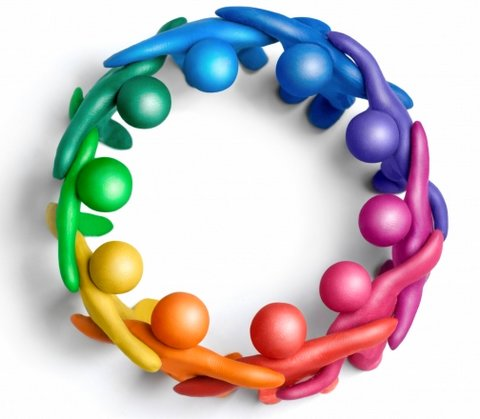
\includegraphics[scale=0.5]{./Ressources/Images/P2P.png}}
  \date{8 Septembre 2010}

  \begin{document}

  \begin{frame}
  \maketitle
  \end{frame}


  \begin{frame}
  \tableofcontents
  \end{frame}

  \section{Introduction}
  \begin{frame}
  	Présentation des points importants à la compréhension du sujet:\\
	\begin{itemize}
		\item Architecture pair à pair Vs Client-Serveur\\
		\item Définition de l'overlay\\
	\end{itemize}
  \end{frame}

  \begin{frame}
	Architecture pair à pair Vs Client/Serveur\\
	\begin{figure}
	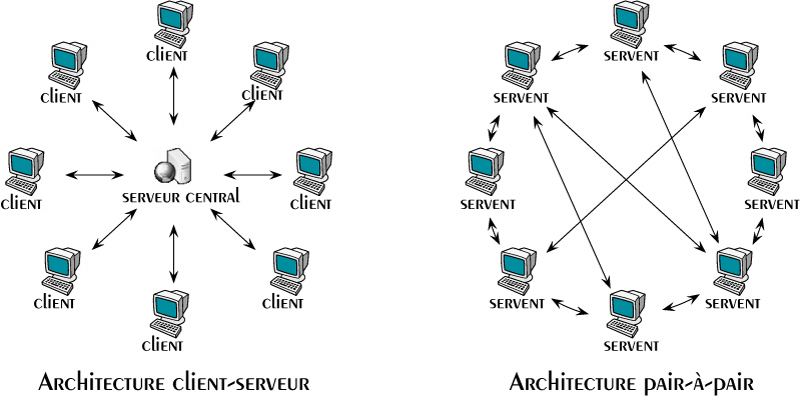
\includegraphics[scale=0.28]{./Ressources/Images/p2p-85145.png}\\
        \label{P2PvsClServ}
        \end{figure}
	\begin{itemize}
		\item Problème du passage à l'échelle de l'architecture Client/Serveur.\\
		\item Solutions p2p existantes pas assez réactives pour assurer une latence suffisante.\\
	\end{itemize}
  \end{frame}
  
  \begin{frame}
	
	\center{Définition de l'overlay}
 	\begin{columns}
          \begin{column}{6,5cm}
	    	\begin{itemize}
		\item Un overlay est un réseau informatique formant un graphe où les liens sont déterminés avec un critère logique.\\
		\item Réseau physique~$\neq$~Réseau virtuel
		\end{itemize}
	  \end{column}
          \begin{column}{5cm}
        	\begin{figure}
        	  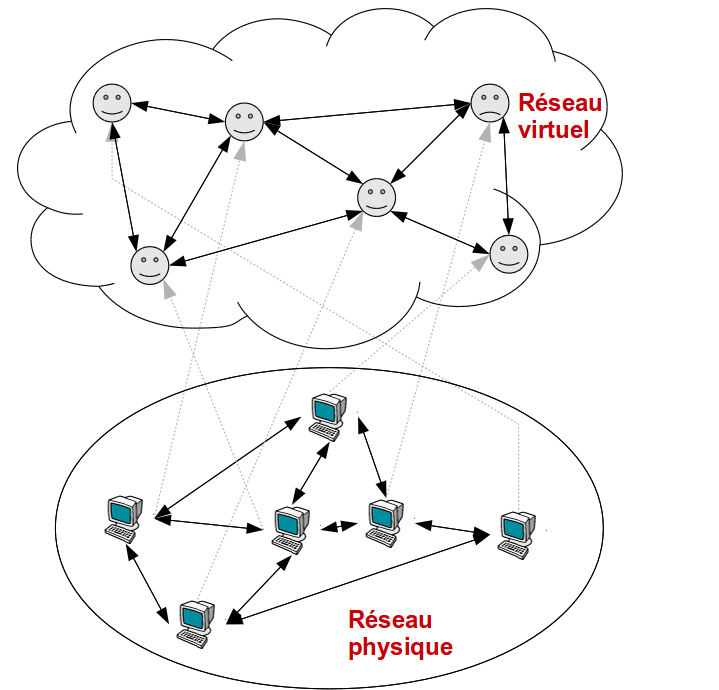
\includegraphics[scale=0.1]{./Ressources/Images/overlay.png}\\
        	  \label{Propa_Algo}
        	\end{figure}
          \end{column}
        \end{columns}
	
  \end{frame}

  \begin{frame}\addtocounter{framenumber}{-1}

        \center{Définition de l'overlay}
        \begin{columns}
          \begin{column}{6,5cm}
                \begin{itemize}
                \item Un overlay est un réseau informatique formant un graphe où les liens sont déterminés avec un critère logique.\\
                \item Réseau physique~$\neq$~Réseau virtuel
                \end{itemize}
          \end{column}
          \begin{column}{5cm}
                \begin{figure}
                  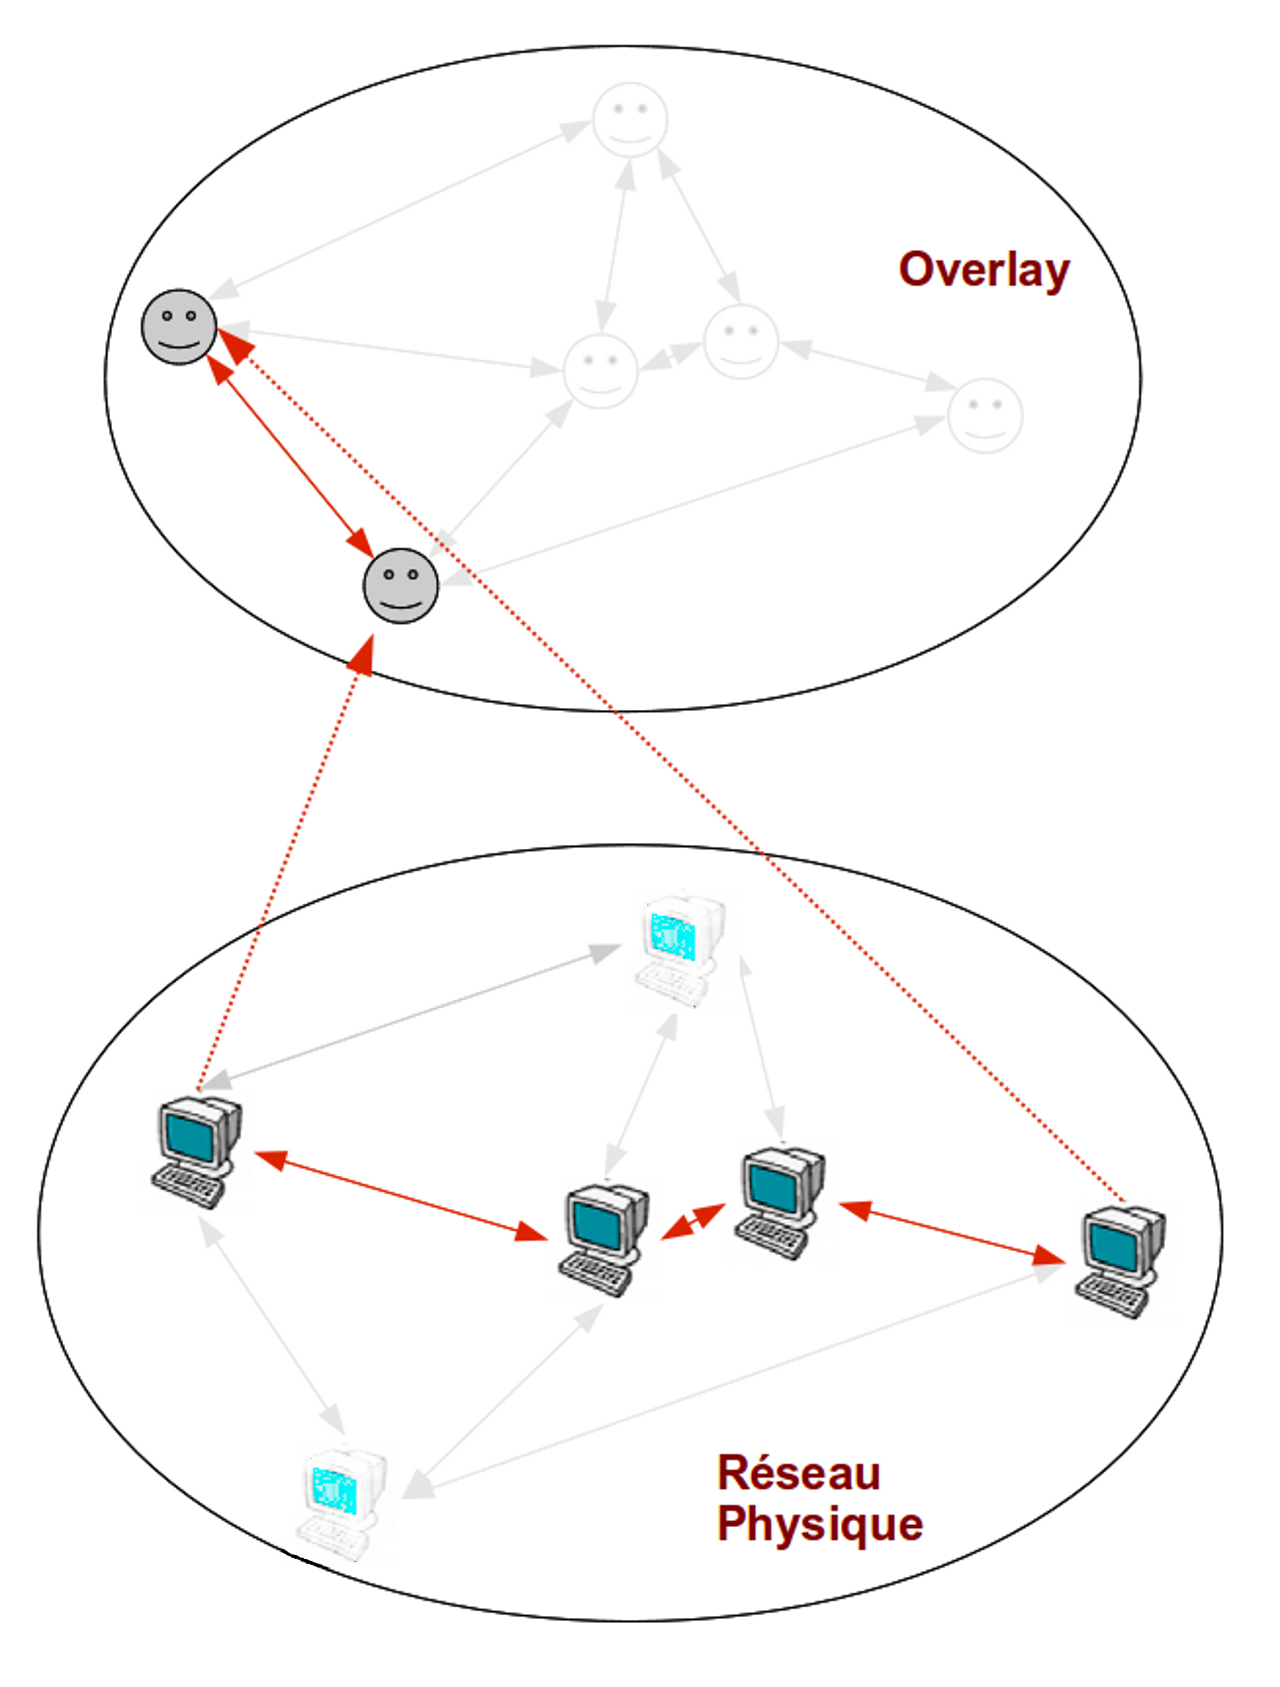
\includegraphics[scale=0.1]{./Ressources/Images/overlay1.png}\\
                  \label{Propa_Algo}
                \end{figure}
          \end{column}
        \end{columns}

  \end{frame}

	
  \section{État de l'art}
  \begin{frame}
	Présentation des  mécanismes importants à la compréhension des solutions proposées:\\
	\begin{itemize}
		\item Solipsis\\
		\item Étude des traces des joueurs de MMOG\\
		\item Blue Banana \\
	\end{itemize}
  \end{frame}

  \subsection{Solipsis}

  \begin{frame}
	%\begin{center}
	%
\includegraphics[scale=0.2]{./Ressources/Images/solipsis.png}\\
	%\end{center}
	%\vspace{4mm}
	\begin{columns}
          \begin{column}{6cm}
	Solipsis:\\
	\begin{itemize}
		\item propose un monde virtuel entièrement décentralisé et scalable.\\
		\item met en place un overlay avec une forte malléabilité applicative.\\
		\tiny{
			\begin{itemize}
				\item Un réseau est malléable si sa topologie est dynamiquement déterminé par l'application reposant sur ce réseau.\\
				%\item La topologie s'adapte à l'application, si deux avatars se rapprochent dans le monde virtuel, les nœuds dans le réseau logique doivent devenir progressivement voisins. \\
			\end{itemize}
		}
	\end{itemize}
	\end{column}
        \begin{column}{4cm}
        \begin{figure}
        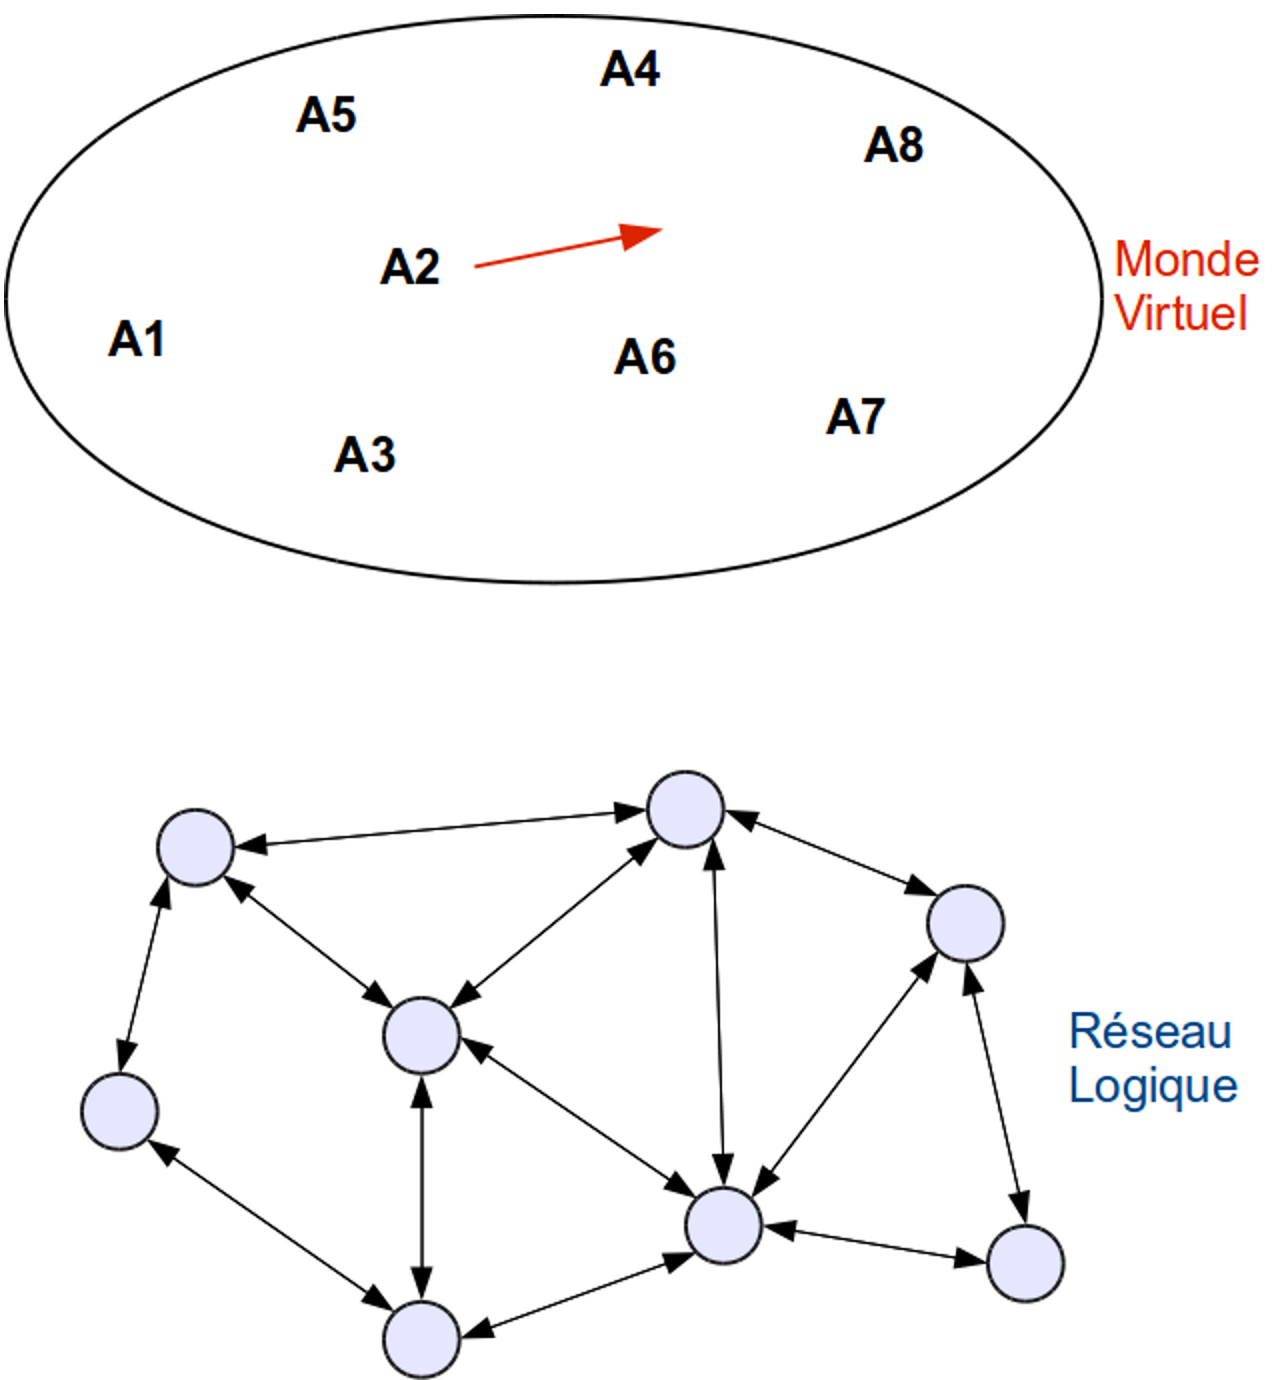
\includegraphics[scale=0.1]{./Ressources/Images/OverlayMalle_et1.png}\\
        \label{Propa_Algo}
        \end{figure}
        \end{column}
        \end{columns}
  \end{frame}

  \begin{frame}\addtocounter{framenumber}{-1}
        %\begin{center}
        %
\includegraphics[scale=0.2]{./Ressources/Images/solipsis.png}\\
        %\end{center}
        %\vspace{4mm}
        \begin{columns}
          \begin{column}{6cm}
        Solipsis:\\
        \begin{itemize}
                \item propose un monde virtuel entièrement décentralisé et scalable.\\
                \item met en place un overlay avec une forte malléabilité applicative.\\
                \tiny{
                        \begin{itemize}
                                \item Un réseau est malléable si sa topologie est dynamiquement déterminé par l'application reposant sur ce réseau.\\
                                %\item La topologie s'adapte à l'application, si deux avatars se rapprochent dans le monde virtuel, les nœuds dans le réseau logique doivent devenir progressivement voisins. \\
                        \end{itemize}
                }
        \end{itemize}
        \end{column}
        \begin{column}{4cm}
        \begin{figure}
        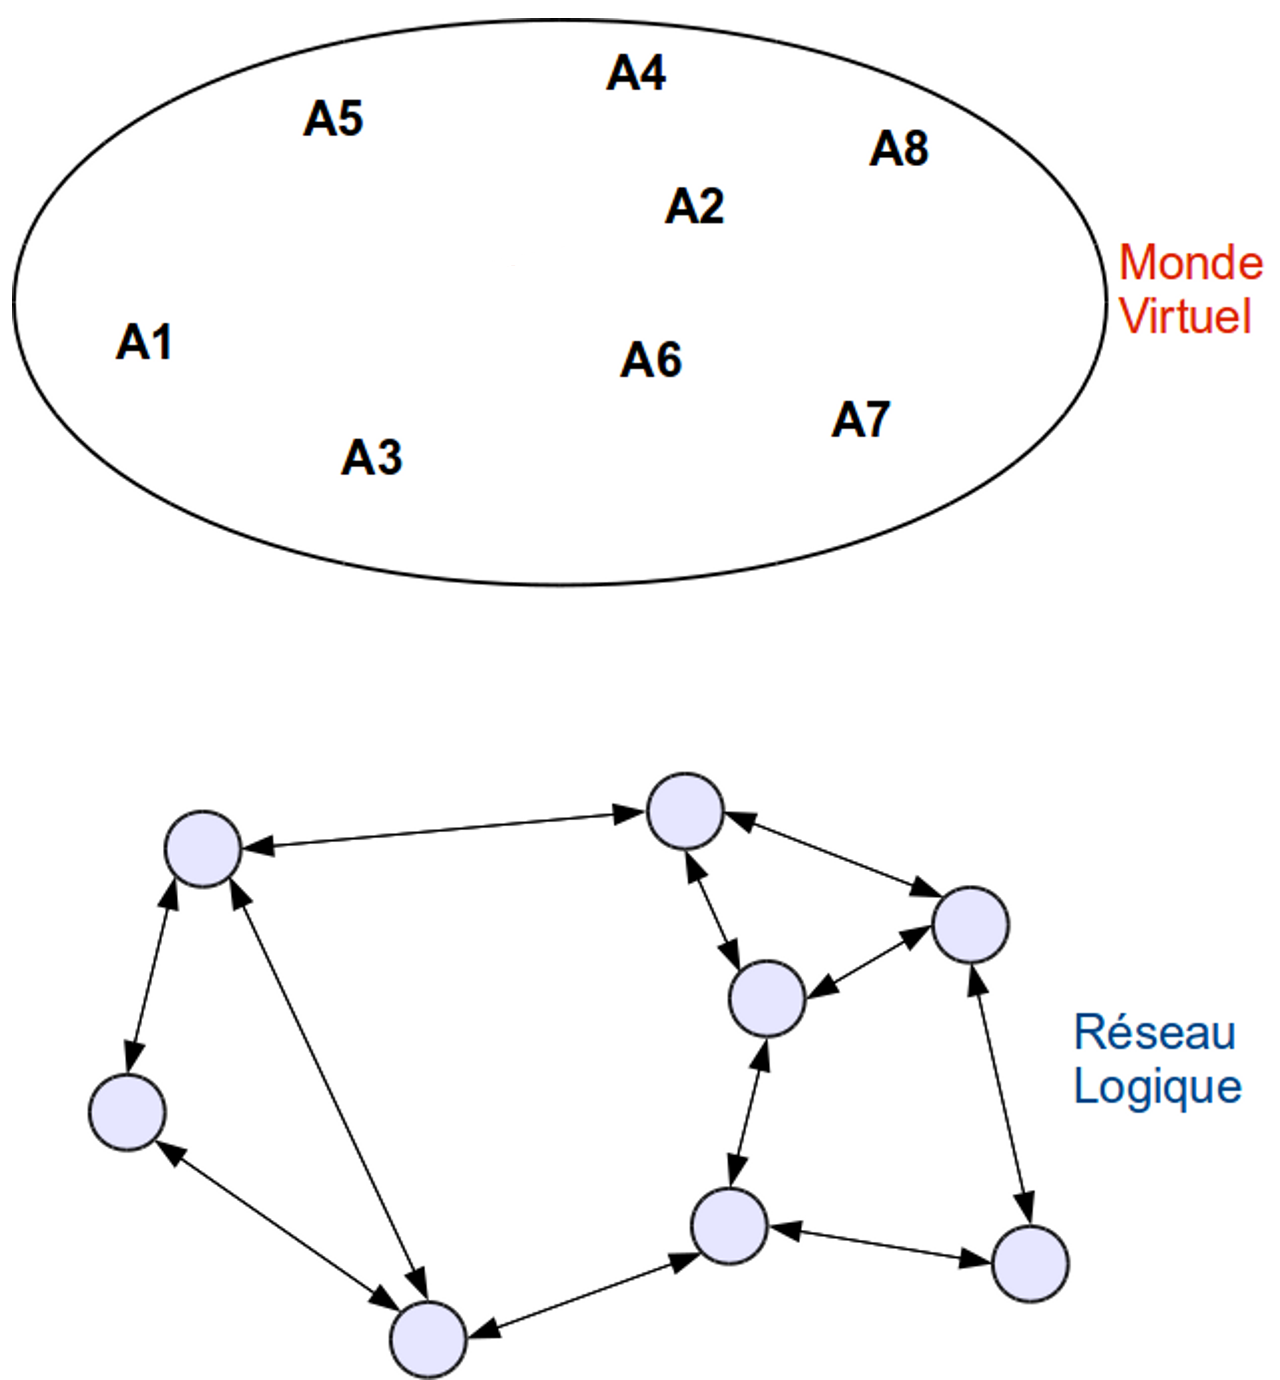
\includegraphics[scale=0.1]{./Ressources/Images/OverlayMalle_et2.png}\\
        \label{Propa_Algo}
        \end{figure}
        \end{column}
        \end{columns}
  \end{frame}


  \begin{frame}
	Solipsis introduit deux propriétés:
	 \begin{columns}
          \begin{column}{6cm}
	   \begin{itemize}
                \item \textit{Connaissance locale:}\\\tiny{
                Une entité doit être connectée avec tous ses plus proches voisins, elle peut connaître des entités en dehors de son environnement virtuel local. Toute entité située à l'intérieur de l'environnement d'une entité doit faire parti des voisins de cette entité.}
                \item \normalsize{\textit{Connectivité globale:}}\\\tiny{
                Toute entité virtuelle doit se trouver à l'intérieur de l'enveloppe convexe contenant l'ensemble de ses voisins logiques. \\}
	   \end{itemize}
	\end{column}
        \begin{column}{4cm}
        \begin{figure}
        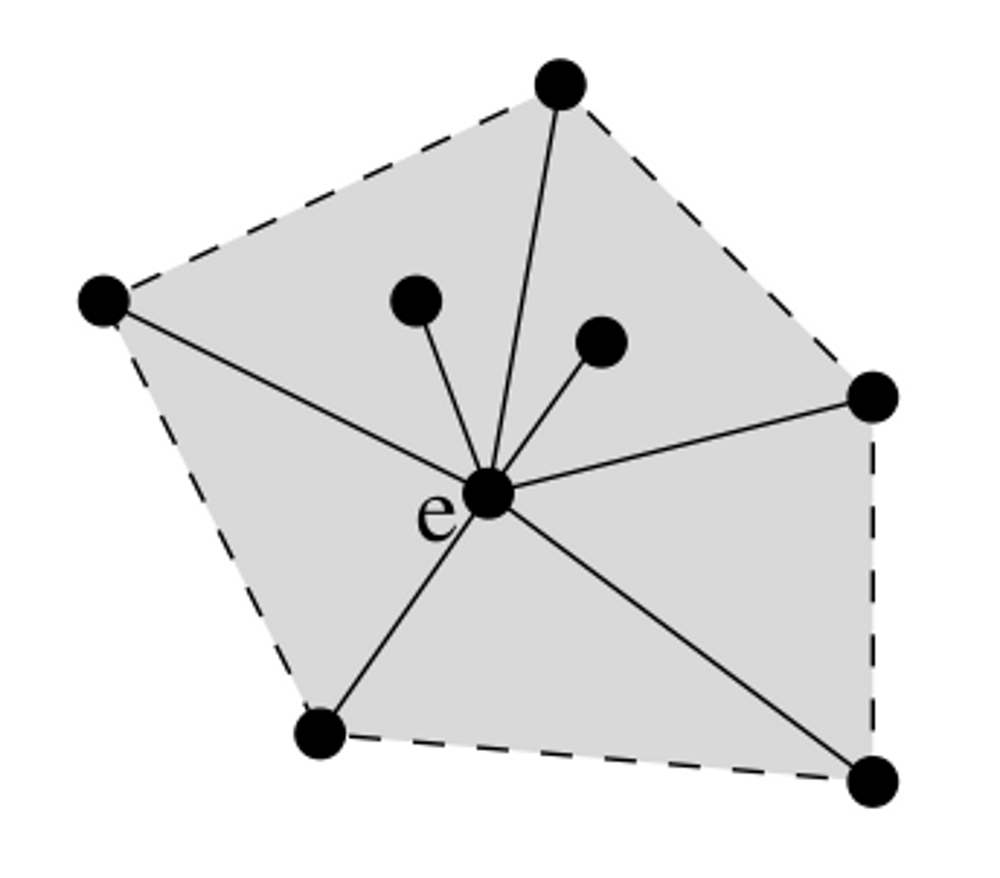
\includegraphics[scale=0.3]{./Ressources/Images/envelop_convex3.png}\\
        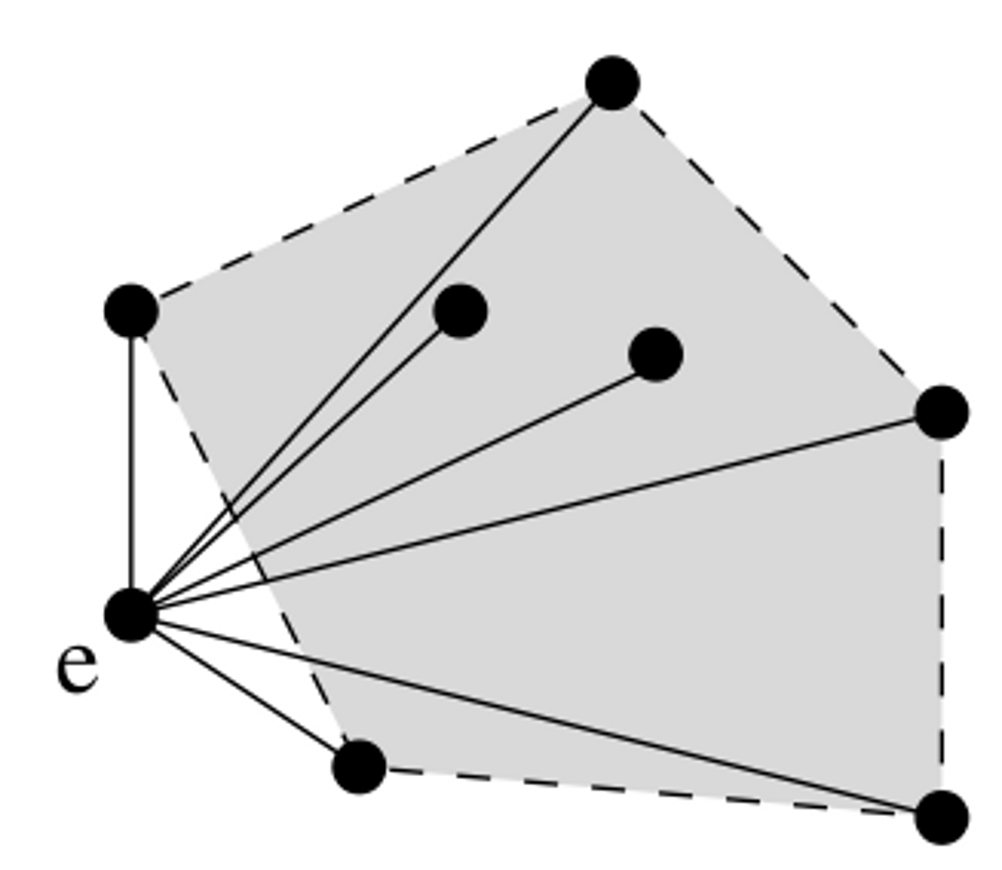
\includegraphics[scale=0.3]{./Ressources/Images/envelop_convex4.png}\\
        \label{Propa_Algo}
        \end{figure}
        \end{column}
        \end{columns}
  \end{frame}

  \subsection{Les traces}
  \begin{frame}
	Des études des traces des joueurs de MMOG, ont permis de faire plusieurs observations sur l'environnement virtuel:
	\begin{itemize}
		\item Présence de zones denses 
		\item Mouvements erratiques dans les zones denses
		\item Mouvements rectilignes et rapides entre les zones denses
	\end{itemize}
	\begin{center}
        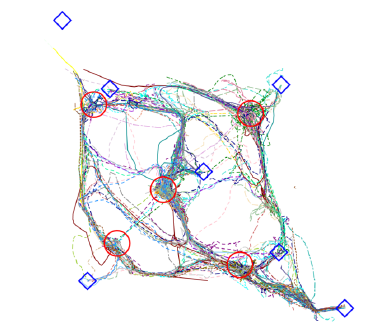
\includegraphics[scale=0.35]{./Ressources/Images/trace.png}\\
        \end{center}
  \end{frame}

  \subsection{BlueBanana}
  \begin{frame}
	 Blue Banana introduit trois états, pour un avatar:
        \begin{itemize}
                \item \textbf{H}(alted): l'avatar est immobile.
                \item \textbf{T}(ravelling): l'avatar se déplace rapidement sur la carte et il a une trajectoire droite.
                \item \textbf{E}(xploring): l'avatar est en train d'explorer une zone, sa trajectoire est confuse et sa vitesse est lente.
        \end{itemize}
  \end{frame}

  \begin{frame}
	Mise en place d'un mécanisme d'anticipation des mouvements des avatars.
	\begin{columns}
	  \begin{column}{5cm}
		\begin{itemize}
		  \item Si état \textbf{T}, il cherche des nœuds sur sa trajectoire.
		  \item Evaluation du nœud, propagation de la requête.
		  \item Réponse au nœud qui a demandé le préchargement.
		\end{itemize}
	  \end{column}
	\begin{column}{5cm}
	\begin{figure}
        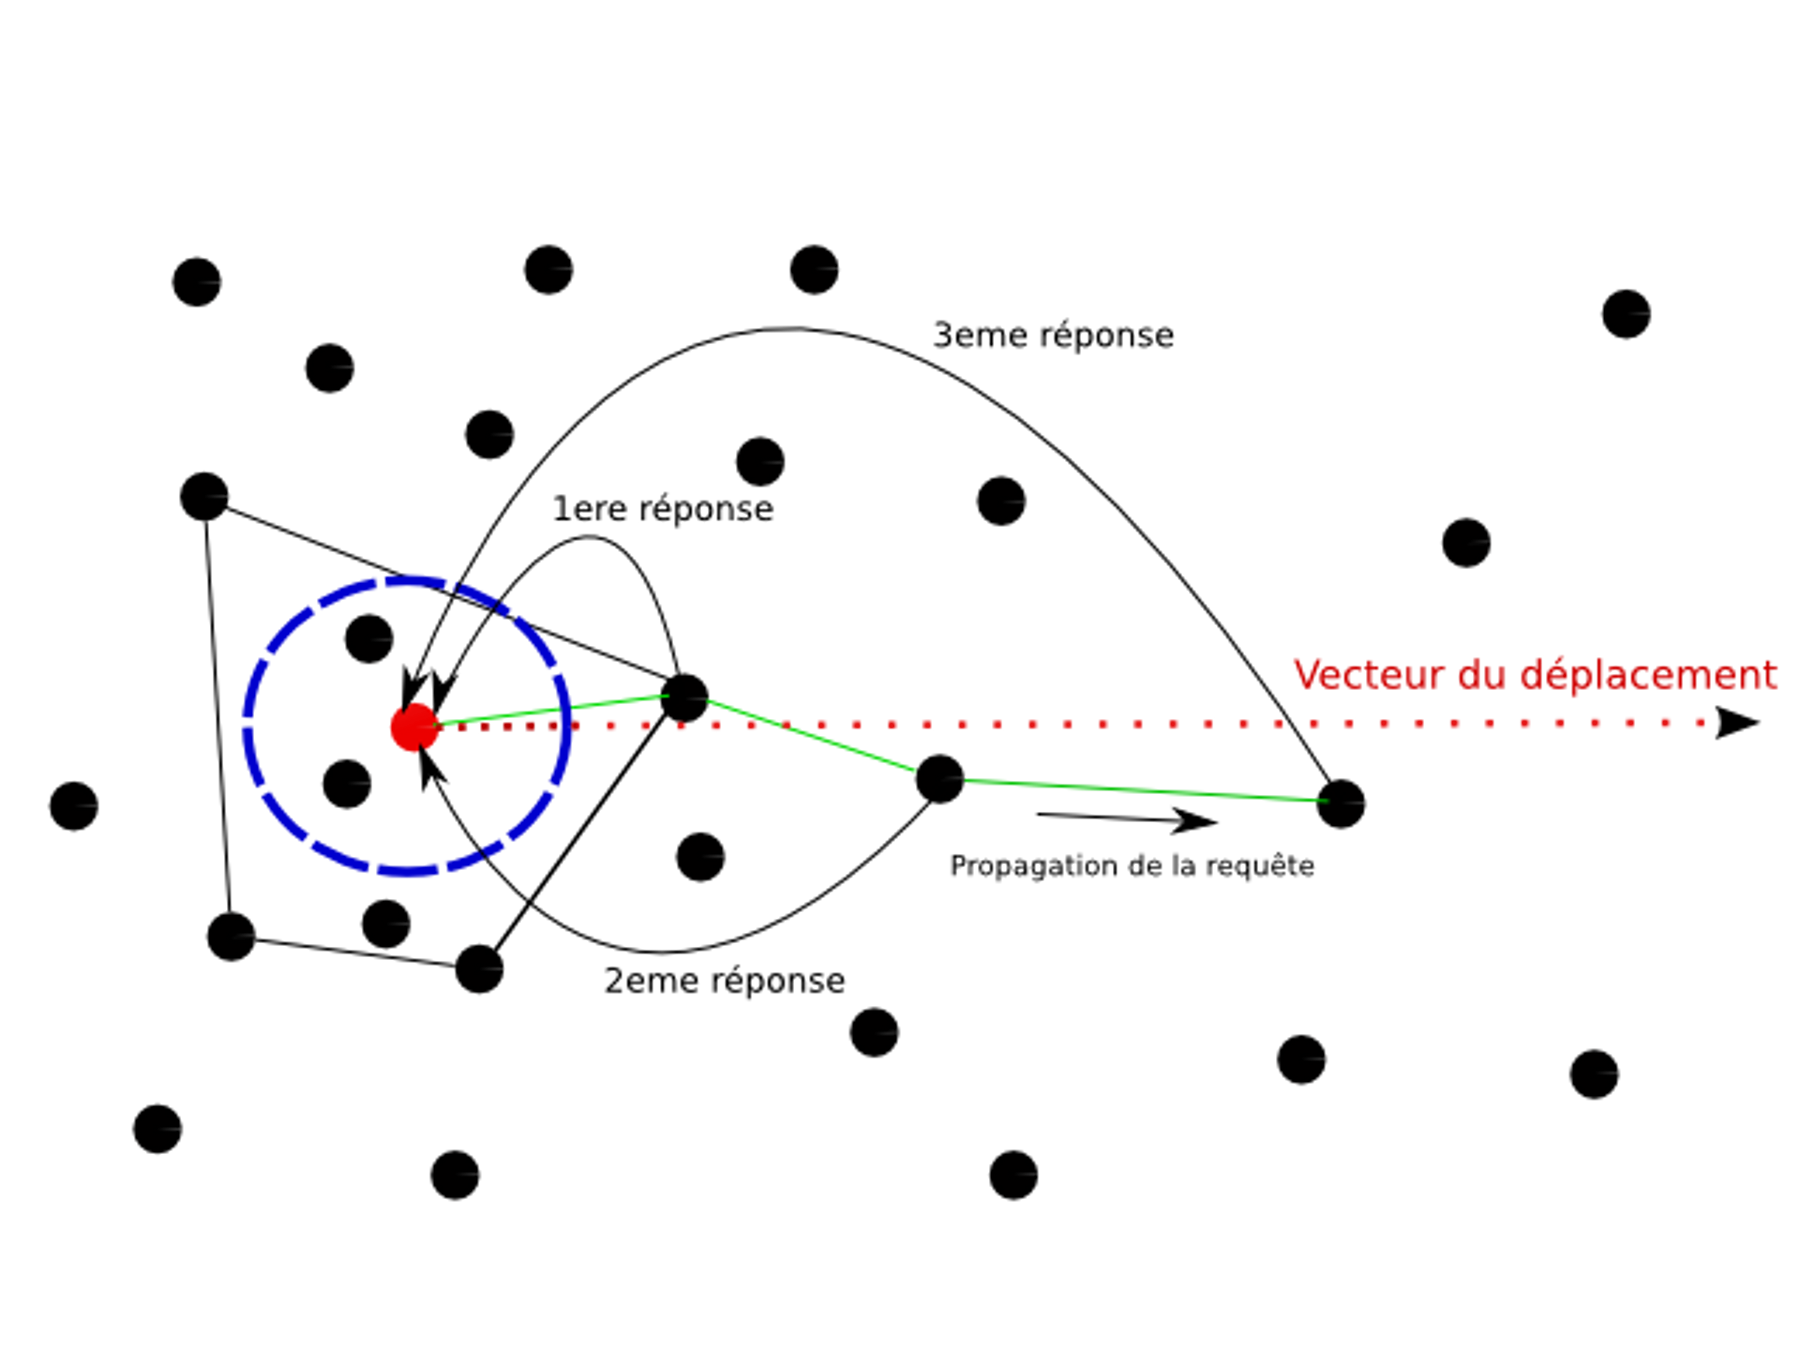
\includegraphics[scale=0.1]{./Ressources/Images/propagation_algo.png}\\
        \label{Propa_Algo}
        \end{figure}
	\end{column}
	\end{columns}
  \end{frame}

  \section{Les améliorations}
  \begin{frame}
	Durant le stage, plusieurs solutions ont été implémentées:
	\begin{itemize}
		\pause\item Le cache pour les zones denses
		\pause\item Le préchargement amélioré des données
	\end{itemize}
	\pause D'autres solutions ont été étudiées, mais sans être implémentées.
	\begin{itemize}
		\item Mouvements de groupe
		\item Connaissance des routes entre les zones denses
	\end{itemize}
  \end{frame}

  \begin{frame}
	Différentes métriques utilisées pour analyser les résultats:
	\begin{itemize}
		\item Nombre de messages à un instant 
		\item Cohérence de la topologie \\ \textit{\footnotesize{Nombre de nœuds dans la zone de connaissance mais pas dans l'ensemble des voisins}}
	\end{itemize}
	\vspace{5mm}
	En fonction du degré de mobilité.
  \end{frame}

  \section{Le cache pour les zones denses}
  \begin{frame}
	\center{Le cache pour les zones denses}
	\vspace{1cm}
	\begin{itemize}
		\item Explications du cache pour les zones denses
		\item Les résultats 
		\item Conclusion sur le cache
	\end{itemize}
  \end{frame}
  
  \subsection{Explications du cache pour les zones denses}
  \begin{frame}
	Comment fonctionne le cache?
	\begin{itemize}
 		\item Chaque nœud de l'environnement a un cache.
		\item Il est utilisé seulement par les nœuds en état \textbf{E}(xploring).
		\item Deux types de cache mis en place (retour simple et retour multiple).
	\end{itemize}
  \end{frame}

  \begin{frame}
	Trois types de recherche dans le cache:
	\vspace{3mm}
	\tiny{
	\begin{table}
  		\begin{center}
    		 \begin{tabular}{|c|c|c|c|}
      		 \hline
      		 N & Critère de sélection & Avantages & Inconvénients\\
      		 \hline
        	 1 & Comparaison distances & Simplicité & Distance~$\ne$~utile, aide pas enveloppe\\
        	 2 & Aide enveloppe & + Enveloppe OK & - bon règles Solipsis\\
        	 3 & Zone de connaissance & Simplicité & aide pas enveloppe\\
      		 \hline
    		 \end{tabular}
  		\end{center}
	\end{table}
	}
	\begin{itemize}
		\item La version 3 a été conservée pour les tests finaux.
		\item Une version 4 avec zone de connaissance et aide à l'enveloppe convexe?

	\end{itemize}
	\center{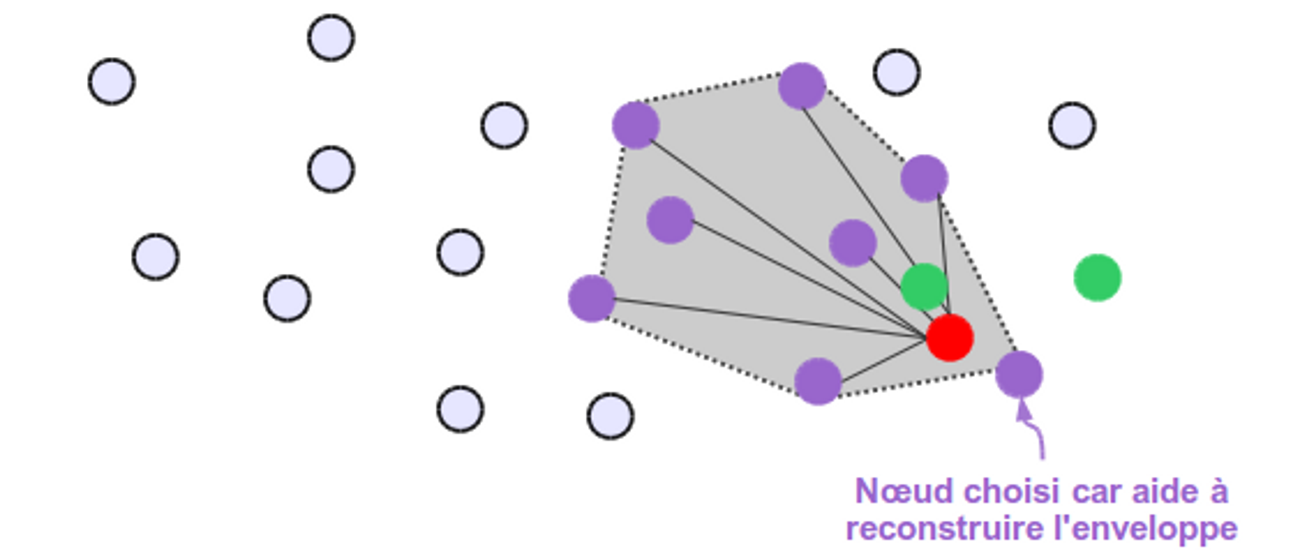
\includegraphics[scale=0.13]{./Ressources/Images/cacheReconstructEnvelop2.png}\\}

  \end{frame}
 
  \begin{frame}\addtocounter{framenumber}{-1}
  	\only{\begin{figure}
        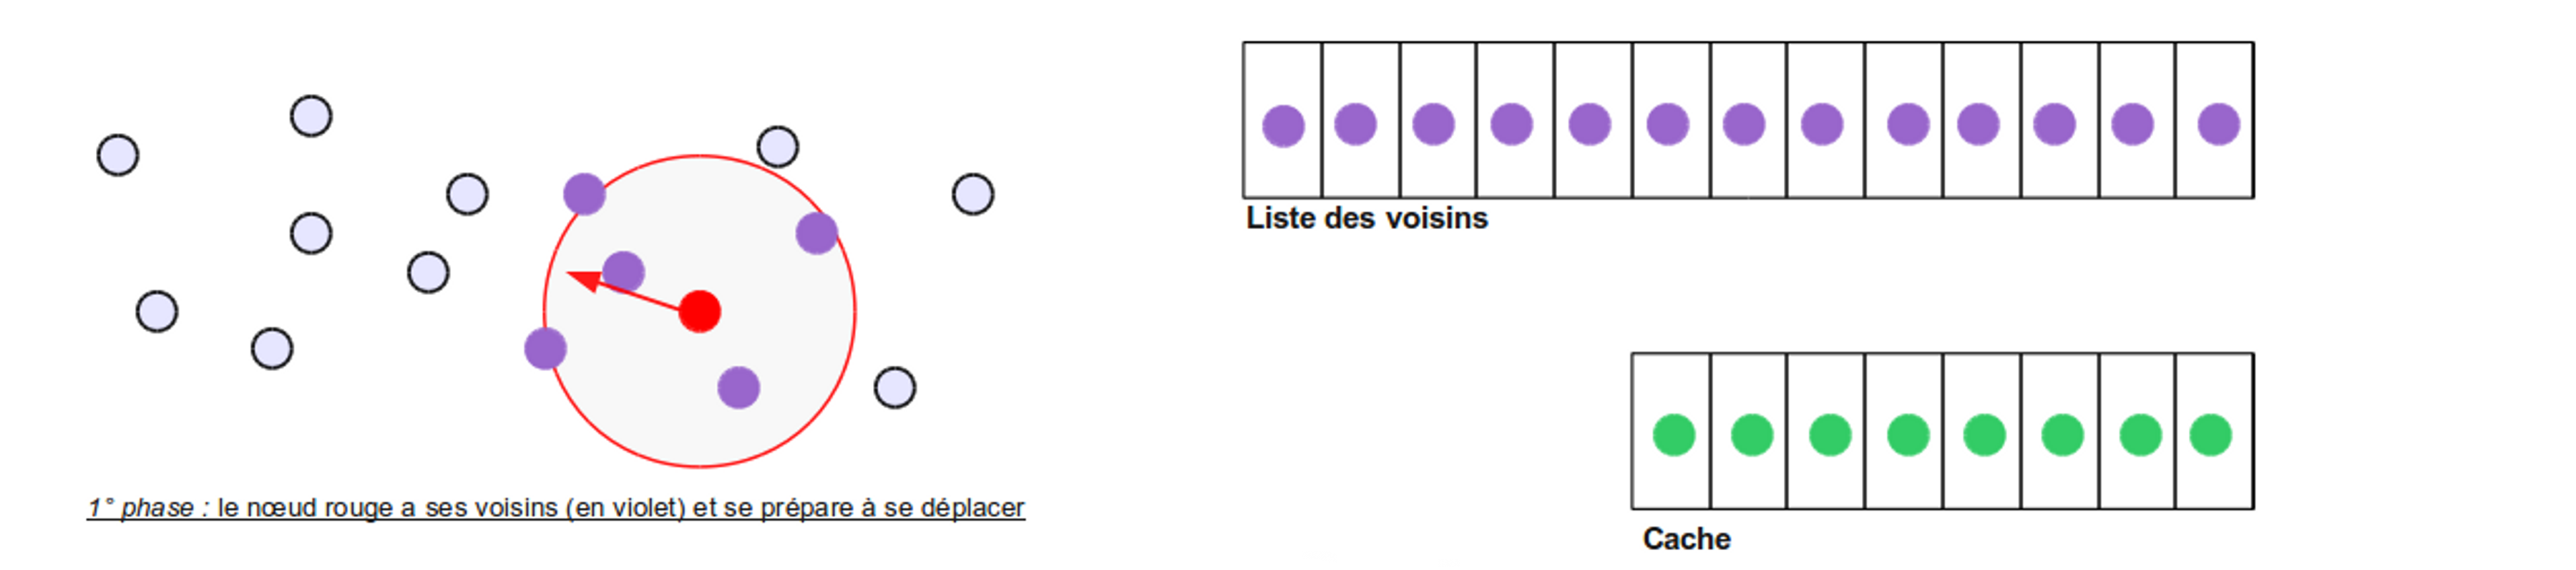
\includegraphics[scale=0.08]{./Ressources/Images/etape1.png}\\
        \label{etape1}
        \end{figure}}
  \end{frame}
	
  \begin{frame}\addtocounter{framenumber}{-1}	
  	\only{\begin{figure}
        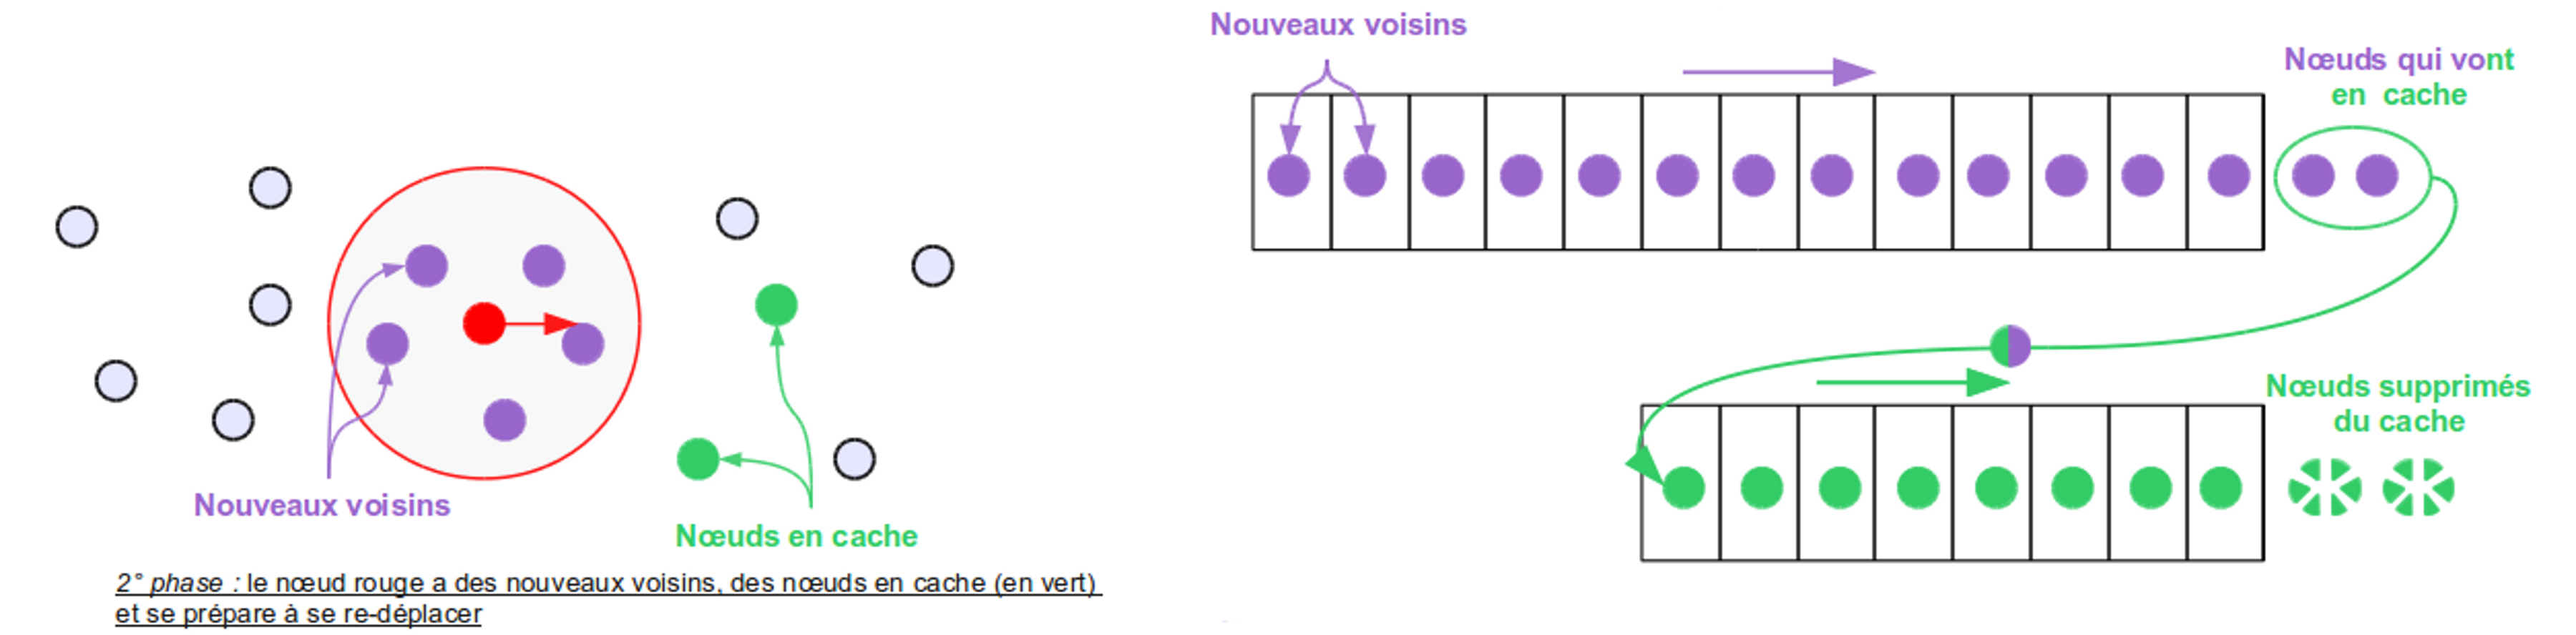
\includegraphics[scale=0.08]{./Ressources/Images/etape2.png}\\
        \label{etape2}
        \end{figure}}
  \end{frame}

  \begin{frame}\addtocounter{framenumber}{-1}
  	\only{\begin{figure}
        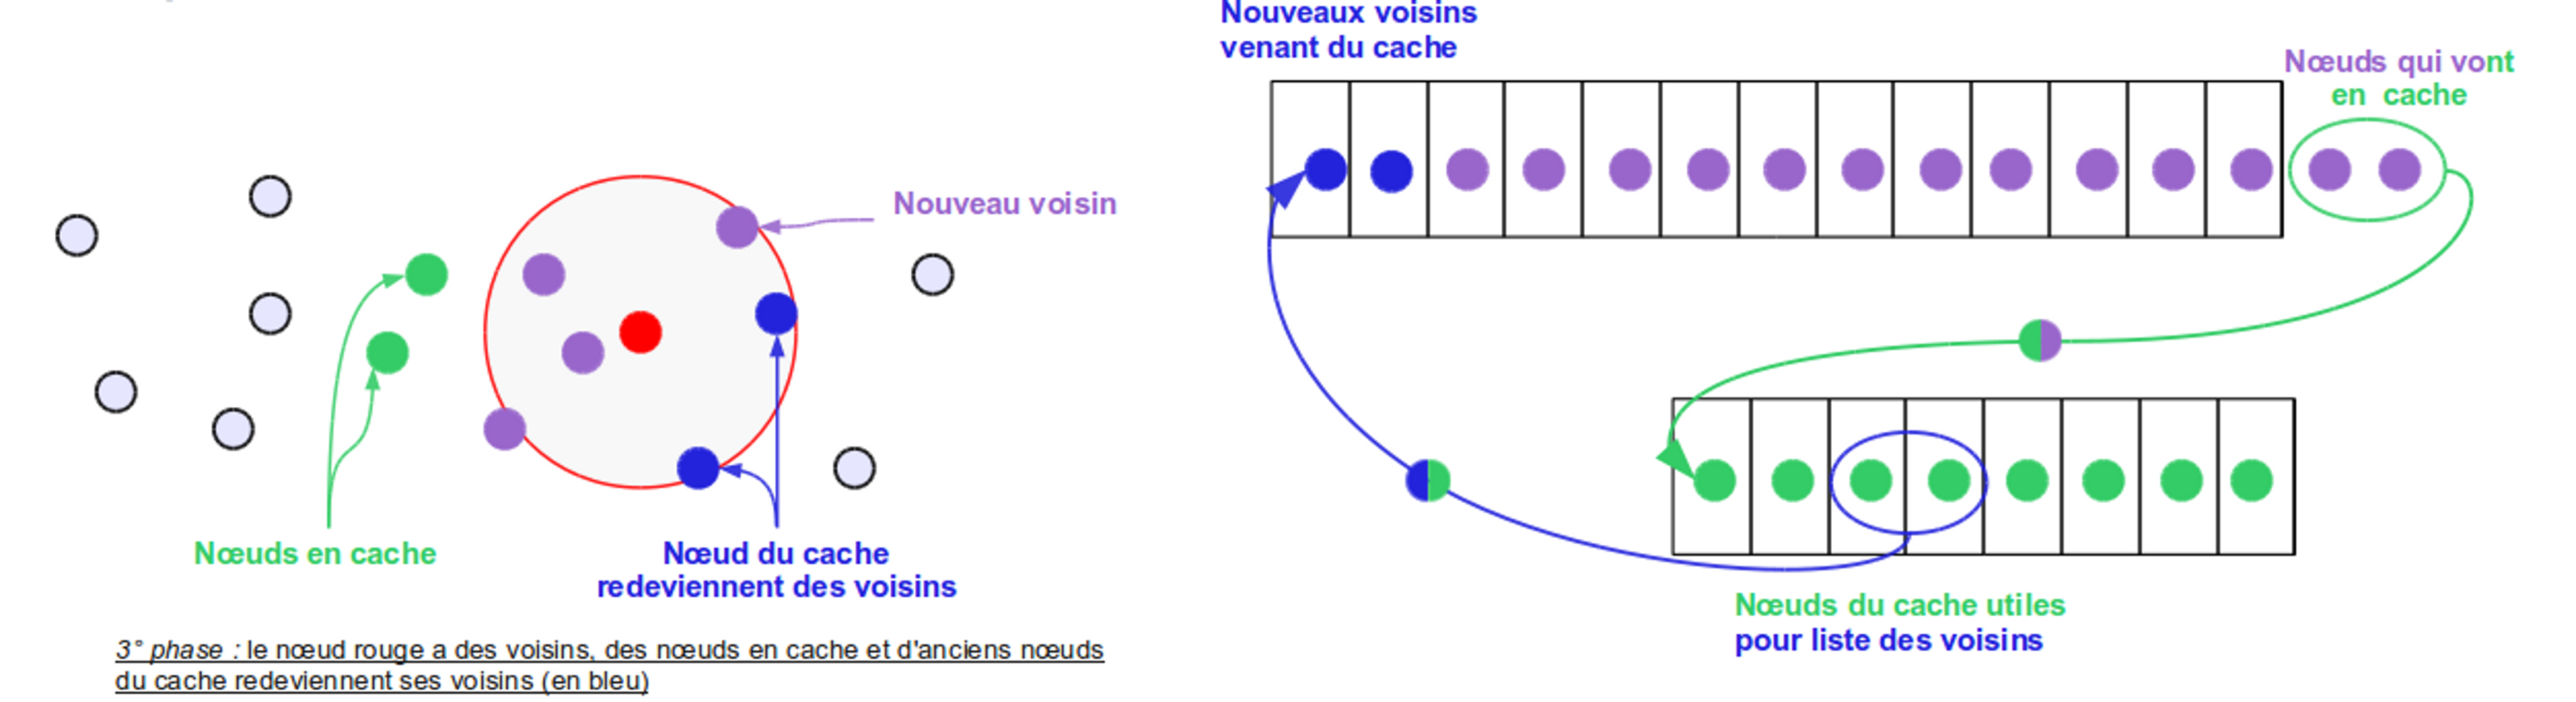
\includegraphics[scale=0.08]{./Ressources/Images/etape3.png}\\
        \label{etape3}
        \end{figure}}


  \end{frame}

  \begin{frame}
	\begin{itemize}
	\item Les données du cache sont mobiles, donc pas à jour.
	\item Différents mécanismes pour le cache:
		\begin{itemize}
		\item Mise à jour des données du cache
		\item Contact un nœud du cache s'il est là depuis longtemps
		\item Aide les nœuds voisins lors de recherche de nœud	
		\end{itemize}
	\end{itemize}
	\footnotesize{
	\begin{table}[!h]
  	\begin{center}
    	\begin{tabular}{|c|c|}
        \hline
      	 Paramètre & Valeur\\
      	\hline
     	 Taille du cache & 25\\
     	 Limite de distance &  1500\\
     	 Limite de temps & 1500\\
     	 Contact Nœud & Faux\\
     	 Mise à jour du cache & Faux\\
     	 Aide aux voisins & Vrai\\
      	\hline
    	\end{tabular}
  	\end{center}
	\end{table}
	}
  \end{frame}

 
  \subsection{Résultats pour le cache}
  \begin{frame}
	\begin{center}
	Nombre de messages 
	\end{center}
	\begin{columns}
         \begin{column}{5cm}
          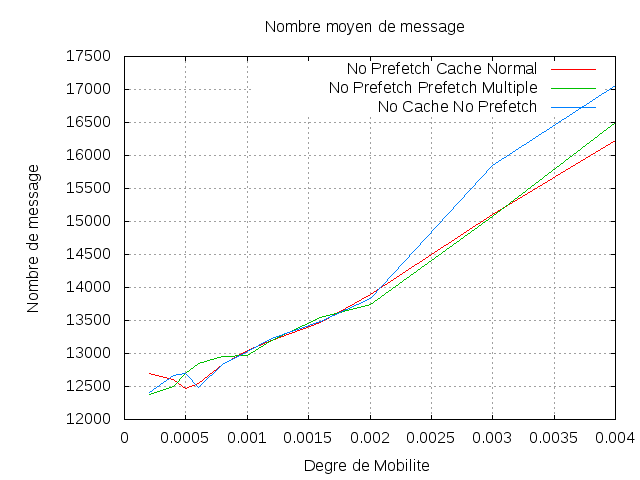
\includegraphics[scale=0.25]{./Ressources/Images/Courbes_Final_Rapport/Nombre_Messages_Caches.png}\\
         \end{column}
         \begin{column}{5cm}
	\footnotesize{ \begin{table}[!h]
                \begin{center}
                \begin{tabular}{|c|c|}
                \hline
                Solution & Nombre de messages \\
                \hline
                Cache simple &  5\% de msg en moins\\
                Cache multiple &  5\% de msg en moins\\
                \hline
                \end{tabular}
                \end{center}
        \end{table}}
         \end{column}
        \end{columns}
        \begin{itemize}\footnotesize{
                \item Moins de messages le cache s'utilise immédiatement sans message.
        }
        \end{itemize}
  \end{frame}

  \begin{frame}
        \begin{center}
        Cohérence de la topologie
        \end{center}
        \begin{columns}
         \begin{column}{5cm}
          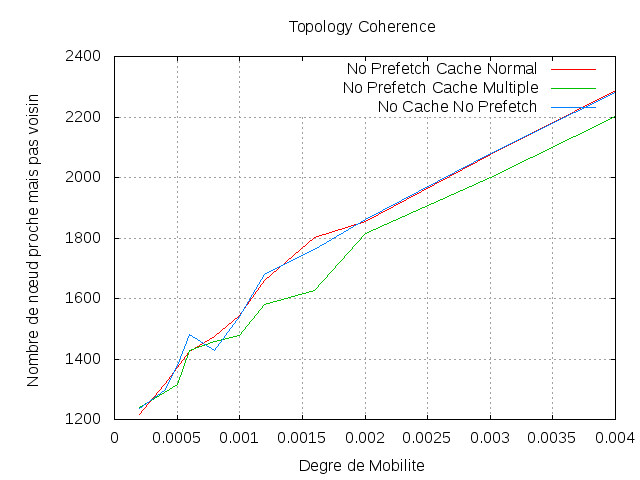
\includegraphics[scale=0.25]{./Ressources/Images/Courbes_Final_Rapport/Topology_Coherence_Caches.png}\\
         \end{column}
         \begin{column}{5cm}
	\footnotesize{
         \begin{table}[!h]
                \begin{center}
                \begin{tabular}{|c|c|}
                \hline
                Solution & Cohérence topologie \\
                \hline
                Cache simple & Équivalente \\
                Cache multiple & 3\% de gains \\
                \hline
                \end{tabular}
                \end{center}
        \end{table}}
         \end{column}
        \end{columns}
        \begin{itemize}\footnotesize{
                \item Gain sur la cohérence de la topologie si retour multiple.
        }
        \end{itemize}
  \end{frame}
	
  \subsection{Conclusion sur le cache des zones denses}
  \begin{frame}
  	La mise en place du cache permet:\\
	\begin{itemize}
		\item d'économiser des messages.\\
		\item d'améliorer la cohérence de la topologie.\\
	\end{itemize}
	\vspace{5mm}
	Amélioration possible en testant toutes les combinaisons de paramètres (mise à jour, contact d'un nœud, taille du cache, etc).\\
  \end{frame}



  \section{L'amélioration du préchargement}
  \begin{frame}
	\center{L'amélioration du préchargement}
	\vspace{1cm}
	\begin{itemize}
		\item Explications sur l'amélioration du préchargement
		\item Les résultats 
		\item Conclusion 
	\end{itemize}
  \end{frame}

  \subsection{Explications sur l'amélioration du préchargement}
  \begin{frame}
	\begin{columns}
        \begin{column}{7cm}
	\textbf{Situation:} Le préchargement de Blue Banana prend tous les nœuds, à bonne distance, dans le cône. Amélioration de la cohérence de la topologie avec un léger surplus de messages.\\
	\vspace{5mm}
	\textbf{Problème:} Des nœuds inutiles sont préchargés.\\
	\vspace{5mm}
	\textbf{Solution:} Choisir plus finement les nœuds qui vont être sélectionnés.\\
	\vspace{5mm}
	\textbf{Comment:} Regarder la direction des nœuds et leur vitesse.\\
         \end{column}
         \begin{column}{3cm}
          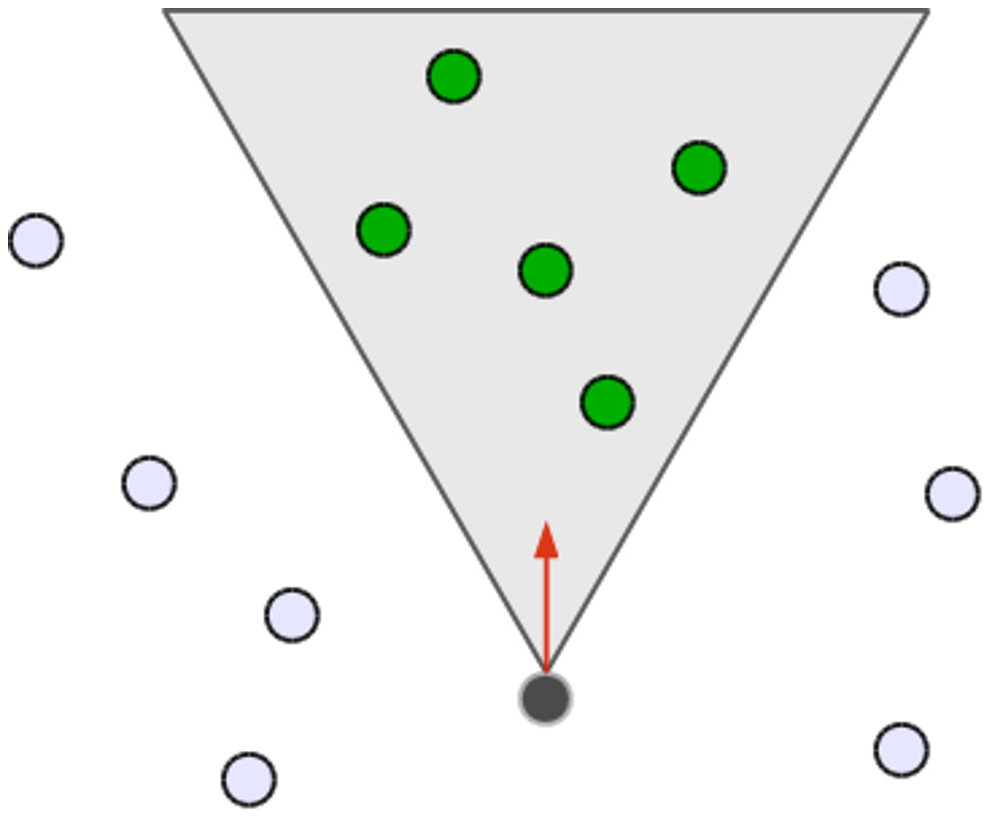
\includegraphics[scale=0.1]{./Ressources/Images/prefetchNormal.png}\\
         \end{column}
        \end{columns}
  \end{frame}

  \begin{frame}
	\begin{columns}
         \begin{column}{5cm}
	 Préchargement amélioré:
          \begin{itemize}
		\item précharger les nœuds qui vont dans le même sens
		\item éviter de précharger des nœuds qui viennent vers le nœud courant avec une vitesse élevée
		\item éviter de précharger des nœuds qui s'écartent du cône
	  \end{itemize}
	 \end{column}
         \begin{column}{6cm}
          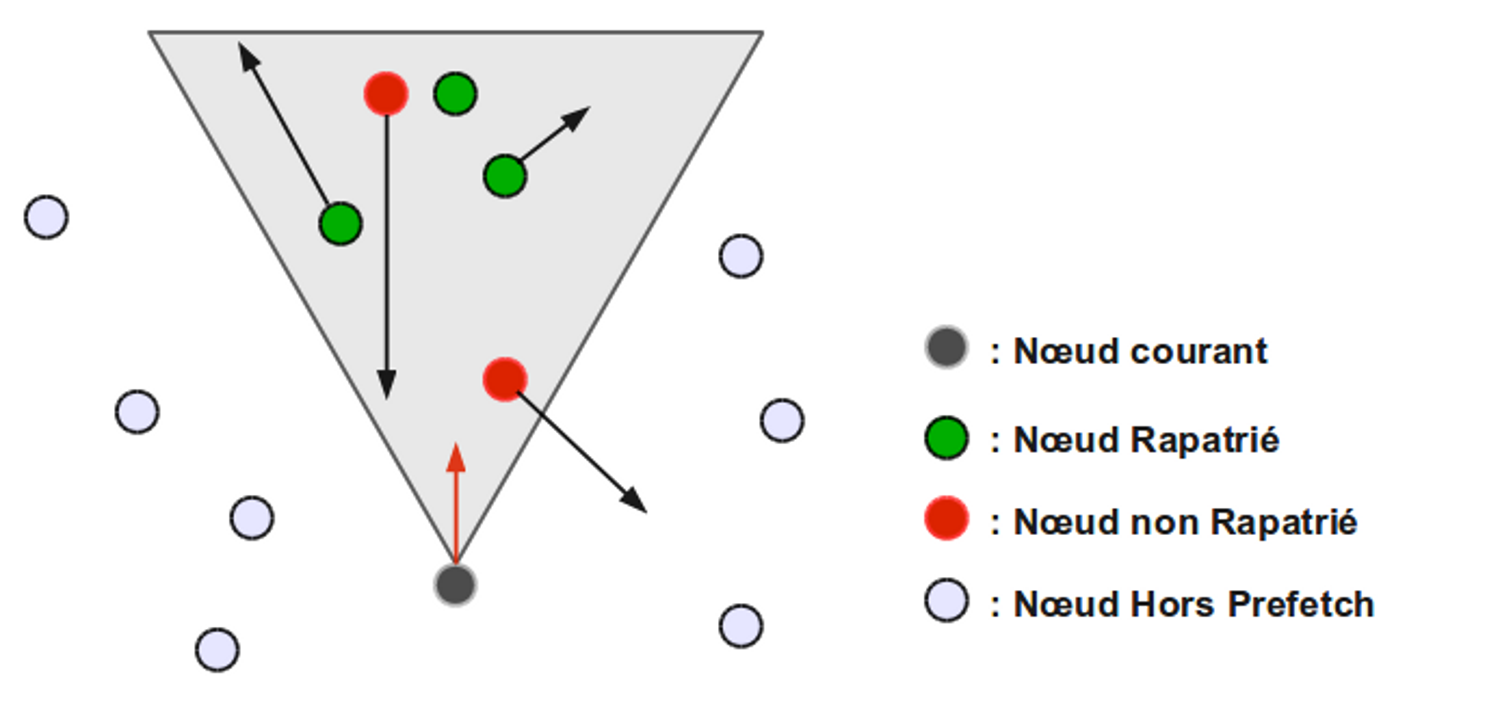
\includegraphics[scale=0.11]{./Ressources/Images/prefetchaV1.png}\\
         \end{column}
        \end{columns}

  \end{frame}
	
  \subsection{Résultats pour l'amélioration du préchargement}
  \begin{frame}
	\begin{center}
	Nombre de messages 
	\end{center}
	\begin{columns}
         \begin{column}{5cm}
          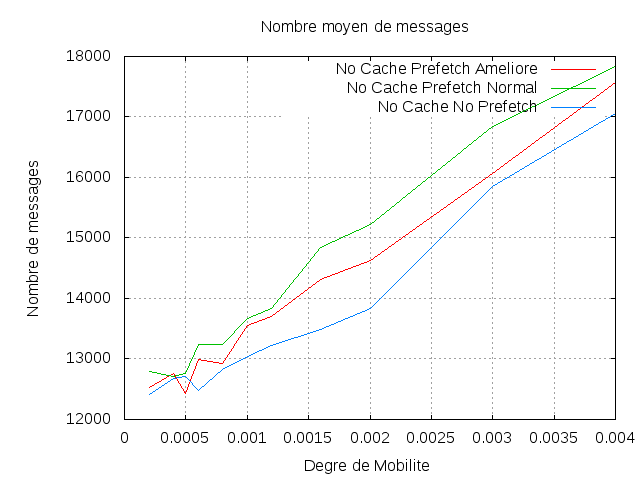
\includegraphics[scale=0.25]{./Ressources/Images/Courbes_Final_Rapport/Nombre_Messages_Prefetchs.png}\\
         \end{column}
         \begin{column}{5cm}
		\begin{table}[!h]
                \begin{center}
                \begin{tabular}{|c|c|}
                \hline
                Solution & Nombre de messages \\
                \hline
                Normal &  8\% de msg en plus\\
                Amélioré &  4\% de msg en plus\\
                \hline
                \end{tabular}
                \end{center}
        \end{table}
         \end{column}
        \end{columns}
	\begin{itemize}\footnotesize{
		\item Gain en terme de messages car préchargement plus efficace, et donc moins de recherche de voisins.
		}
	\end{itemize}
  \end{frame}
	
  \begin{frame}
        \begin{center}
        Cohérence de la topologie
        \end{center}
        \begin{columns}
         \begin{column}{5cm}
          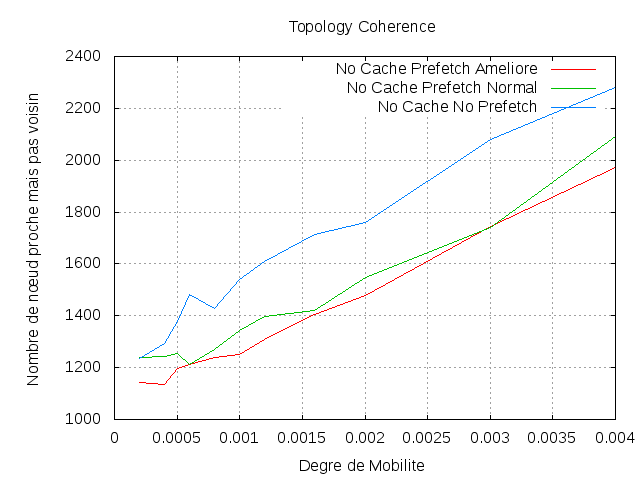
\includegraphics[scale=0.25]{./Ressources/Images/Courbes_Final_Rapport/Topology_Coherence_Prefetchs.png}\\
         \end{column}
         \begin{column}{5cm}
		\begin{table}[!h]
                \begin{center}
                \begin{tabular}{|c|c|}
                \hline
                Solution & Cohérence topologie \\
                \hline
                Normal & 15\% de gains \\
                Amélioré & 16\% de gains \\
                \hline
                \end{tabular}
                \end{center}
        \end{table}
         \end{column}
        \end{columns}
	\begin{itemize}\footnotesize{
		\item Léger gain sur la cohérence de la topologie car élimination du préchargement de certains nœuds inutiles.
		}
	\end{itemize}
  \end{frame}

  \subsection{Conclusion sur l'amélioration du préchargement}
  \begin{frame}
	Notre amélioration du préchargement permet:
	\begin{itemize}
		\item d'économiser des messages par rapport au préchargement normal.\\
		\item d'améliorer légèrement la cohérence de la topologie.\\
	\end{itemize}
	\vspace{5mm}
	Possibles améliorations du préchargement en regardant d'autres paramètres, comme la distance avec les nœuds.
  \end{frame}
	
  
  \section{Conclusion}
  \begin{frame}
	\begin{itemize}
	\item Les solutions ont permis d'améliorer la réactivité des réseaux pair à pair pour les MMOGs.\\
	\item Meilleure cohérence de la topologie et moins de message que dans Blue Banana.
	\item Perspectives :\\
	\begin{itemize}
	\footnotesize{
	\item Meilleure utilisation des mécanismes du cache
	\item Amélioration du préchagement
	\item Mouvements de groupe\\
	\item Route entre les zones denses.\\}
	\end{itemize}
	\end{itemize}
  \end{frame}
	

  \begin{frame}
	\begin{center}
	Merci.\\
	\vspace{1cm}	
	Questions?
	\end{center}
  \end{frame}  

  \end{document}
